\chapter{字符串编辑距离}

\begin{introduction}
	\item 问题引入
	\item 相关概念
	\item 算法思想
\end{introduction}

\section{问题引入}
如何定义两个字符串的距离呢?ocurrance和occrrence有多大的区别呢?下面我们将讨论两个字符串的距离问题。
\section{相关概念}
\begin{definition}{匹配M}{matching}
	字符串X有$x_1$到$x_n$共n个字符,字符串Y有$y_1$到$y_m$共m个字符。X和Y之间存在一个匹配M,其满足:$if (i,j) \in M, (l,k)\in M, i<l iff j<k$。
\end{definition}

%距离代价:

%$\alpha_{xy}$ :两个不同的字符x和y相匹配的代价,则$\alpha_{xy}=0$.

%$\delta$ :每存在一个没有被选择的字符就会多一个$\delta$.

%总距离代价:所有$\delta$ 和 $\alpha$ 的和。

\begin{definition}{距离代价}{penalty}
	$\alpha_{xy}$:两个不同的字符x和y相匹配的代价,则$\alpha_{xy}=0$.
	
	$\delta$:每存在一个没有被选择的字符就会多一个$\delta$.
	
	总距离代价:所有$\delta$ 和 $\alpha$ 的和。
\end{definition}

示例:

\begin{figure}[htb]
	\centering
	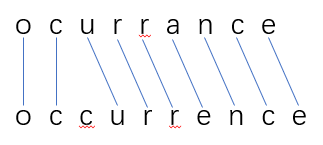
\includegraphics[scale=0.6]{image/connect1.png}
	\caption{字符串匹配}\label{fig:connect1}
\end{figure}
如上图所示,其中的总距离代价为$\alpha_{ae} + \delta$

\section{算法思想}
从后往前推:

bopt (i,j):字符串$x_1,\ldots,x_i$和$y_1,\ldots,y_j$之间的最佳匹配
\begin{equation}
	bopt (m,n)=\begin{cases}
		bopt(m-1,n-1)+\alpha_{x_m y_n} & \text{$x_m$和$y_n$ 相连} \\
		bopt (m-1,n)+\delta            & \text{$x_m$跳过}         \\
		bopt (m,n-1)+\delta            & \text{$y_n$跳过}
	\end{cases}
\end{equation}

从前往后推:

fopt (i,j):字符串$x_i,\ldots,x_m$
和
$y_j,\ldots,y_n$
之间的最佳匹配
\begin{equation}
	fopt (1,1)=\begin{cases}
		fopt(2,2)+\alpha_{x_1 y_1} & \text{$x_1$和$y_1$ 相连} \\
		fopt (2,1)+\delta          & \text{$x_1$跳过}         \\
		fopt (1,2)+\delta          & \text{$y_1$跳过}
	\end{cases}
\end{equation}
初始化:
$bopt (i,0) = \delta_i  $    $bopt (0,i) = \delta_j$

构造图:

\begin{figure}[htb]
	\centering
	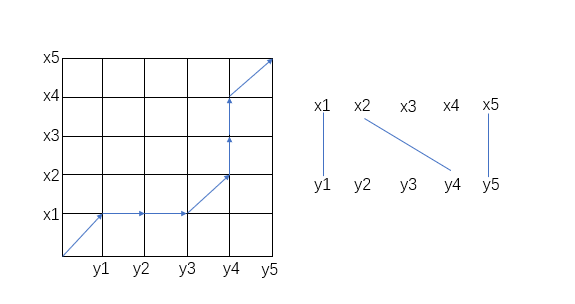
\includegraphics[scale=0.6]{image/connect2.png}
	\caption{构造图}\label{fig:connect2}
\end{figure}
按图构造方法如图所示
